\chapter{Discussion}
\label{sec:discussion}

\section{Realizing Proposed Mechanisms in Contemporary Edge Computing Offerings}
In this chapter we discuss how the proposed mechanisms can be incorporated into the Edge platform offerings at present, and how they interact with the different stakeholders in the Edge Computing ecosystem.
\subsection{Stakeholders in Edge Computing}
The following stakeholders exist in contemporary Edge Computing offerings:
\par \noindent \textbf{Infrastructure Provider.} The most significant factor that differentiates Edge computing from the existing Cloud computing paradigm is the presence of a large number of geo-distributed infrastructure sites, which can be leveraged to offer compute, storage and networking services. Unlike building datacenters in a remote location, setting up Edge infrastructure capabilities is more complicated. This is because, firstly, multiple sites of real-estate have to be purchased in an urban area and power and network connectivity have to be ensured, all of which are expensive and cumbersome to manage. Secondly, since users of Edge applications would inevitably connect to the applications running on these sites through a telecommunication network, the Edge sites should be peered efficiently with the telecom network to avoid high access latencies, despite geographical proximity. Hence, there is a high bar for entry for newcomers in the Edge computing arena.
\par Fortunately, there are existing organizations who already manage such a geo-distributed infrastructure for their own purposes - telecommunication providers, such as AT\&T and Verizon. They operate a large number of geo-distributed central offices which are stocked with network functions (NFV) or custom hardware that enable cellular connectivity. Recently, they have been opening up their infrastructure to be used for hosting Edge computing platforms. For instance, Verizon has partnered with Amazon Web Services to offer AWS Wavelength, which is an offering that provides AWS compute and storage services from Edge infrastructures located in several metropolitan areas in the USA \cite{aws_wavelength}. Similarly, AT\&T has partnered with Microsoft to provide Edge computing services \cite{att_microsoft}. Since these Edge sites are within the network of telecommunication providers, application clients would not have to pay extra latency overhead to communicate with them. 
\par There is a different flavor of infrastructure providers entering the Edge ecosystem. Examples of such infrastructure providers are Vapor IO \cite{vaporio} and Edge Micro \cite{edge_micro}. These organizations build up facilities to serve as Edge sites and ensure efficient peering to network providers serving users closeby. Because of efficient peering, they are able to offer low-latency access to clients that are connect to them through other network service providers.

\par \noindent \textbf{Platform Providers.} These are organizations that utilize the infrastructure owned by Infrastructure Providers to run their application platform/middleware. Examples of platform providers are Amazon Web Services and Microsoft Azure, who already have experience in providing such middleware in the Cloud computing space. The middleware provided by them consists of several platform services that the applications can utilize, such as execution runtimes for applications, key-value stores for data storage and message queues for communication. Usually the same platform services that are offered by the provider in the cloud are made available at the Edge. Examples of such offerings are AWS Wavelength, Microsoft Azure Edge Zones, and Azure IoT Edge.

\par \noindent  \textbf{Application Developer. } The application developer utilizes the platform services offered by the platform provider to implement the application logic. 

\begin{figure}
\centering
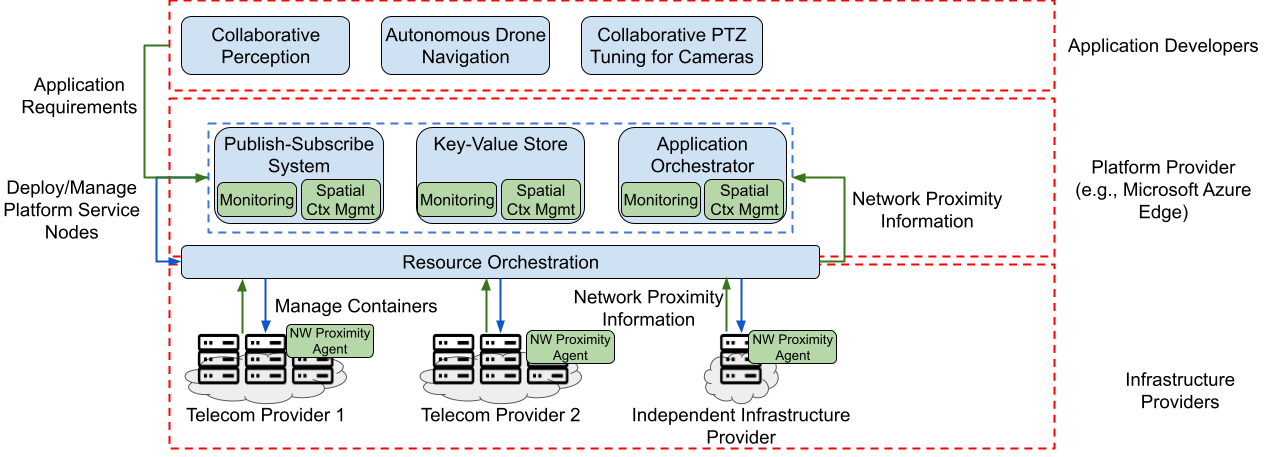
\includegraphics[width=\linewidth]{figures/misc/edge_stakeholders.png}
\caption{\new{Schematic of the various stakeholders in an Edge computing environment and their interactions with one another.}}
\label{fig:edge_stakeholders}
\end{figure}

\subsection{Dependencies of Proposed Mechanisms on Stakeholders}
We now discuss the kinds of dependencies that the proposed mechanisms have on the stakeholders of the Edge computing ecosystem. We will break down each mechanism into its constituent components and discuss which stakeholder manages that component.
\subsubsection{Dynamic Spatial Context Management Mechanism}
The Dynamic Spatial Context Management mechanism consists of two main components -- (1) the spatial partitioning metadata managed by the control policy; and (2) the client library that maintains a cache of the current spatial tile and reports client location to the spatial partitioning metadata component. The spatial partitioning metadata has to be maintained within the control plane of the platform service that uses the mechanism. The client library of the mechanism needs to be incorporated into the client library of the platform service.
\subsubsection{Network Proximity Estimation}
The Network Proximity Estimation mechanism consists of three main components -- (1) Edge Gateways; (2) Network Coordinate Agents on clients; and (3) Network Coordinate Agents on Edge sites. The Edge Gateways will have to be set up and maintained by the infrastructure providers as it is dependent on the network connectivity of clients and independent of the deployment of platform services. Network coordinate agents on the Edge sites would be managed by the infrastructure provider or the platform provider. In case they are managed by the platform provider, they would be able to have agents belonging to different infrastructure providers to be part of the same network coordinate cluster. Network coordinate agents on the clients could be a part of the client library of the platform provider itself, e.g., the client SDK of Azure IoT Edge. It could also be a part of the client library of the platform service.

\subsubsection{End-to-End Monitoring}
All components of the end-to-end monitoring mechanism would be deployed on the platform provider, possibly with one instance of the monitoring mechanism for each platform service.

%\section{Divesting Proposed Mechanisms from the In-Context Implementation}

\section{Edge-Centric Architecture of Control-Plane}

The mechanisms proposed in this dissertation aim at aiding the control-plane policies in their decision-making so that the data-plane of the platform services can be optimized for supporting situation-awareness applications. However, a move from the Cloud to the Edge not only affects the data-plane, but also the control-plane. In cloud-based implementations of platform services, the control-plane and data-plane are both resident within the same datacenter, and the latency between them is negligible. However in the Edge setting, these two components are separated potentially by a Wide Area Network. The high network latency between the control and data plane leads to the responsiveness of the platform service to deteriorate.
\par While this is not the focus of this dissertation, we make two specific optimizations in two of the platform services presented here to improve the responsiveness of the control-plane. 

\subsection{Increase Decision-making Autonomy at the Edge}
\oneedge{} considers two classes of applications - \textit{coordinated} and \textit{standalone}. Coordinated applications are those that require multi-client collaboration, and hence scheduling decisions for them are taken in a centralized controller. On the other hand, each instance of a standalone application serves a unique client. Therefore, application placement for a standalone application client can be done independent of other clients. \oneedge{} assigns the responsibility of standalone application placement to the Site Agents themselves, which receive deployment requests directly from the clients. 
\par Through experimental evaluations on real-world workloads in \cite{oneedge}, we have shown that adding autonomy for resource scheduling improves the response time of the control plane. However, this autonomy results in the emergence of multiple writers to the aggregate infrastructure state maintained by the control plane, which needs to be consistent. One technique that allows high control-plane throughput in the presence of concurrent autonomous updates to the aggregate state by Site Agents is to maintain an eventually consistent view of the aggregate state at the central controller and use it to optimistically make scheduling decisions. These decisions then need to be verified against the remaining resource capacity at the Edge sites during Transaction Executor's operation. If the target Edge sites do not have enough spare capacity to carry out the scheduling decision, the decision is rolled back, aggregate state updated and the scheduling is redone. We have shown that the probability of conflicts between the central controller's and site agents' updates is low, which allows such a design to achieve high throughput and avoid overhead of rollback and rescheduling \cite{oneedge}.

\subsection{Improve Coordination between Control-Plane and Data-Plane}
One of the important objectives of platform services serving situation-awareness applications is their ability to respond to performance violations by performing reconfigurations with agility. Such reconfigurations typically require multiple rounds of communication with the central control-plane and the data-plane components involved. Due to the high WAN latency between control and data-plane components, this process is slowed down, leading to the clients continuing to face performance violations for an extended period of time. \epulsar{} tackles this problem by making the communication between control and data-plane asynchronous, so that the multiple rounds of communication can proceed in parallel, thereby shortening the time required for performing the reconfiguration \cite{epulsar}.


%\section{Lessons Learned}
%\subsection{}
%\subsection{}